\documentclass[aspectratio=169, table, 12pt]{beamer}

\usepackage{colortbl}
\usepackage{xcolor}
\usepackage{listings}
\usepackage{tabularx}
\usepackage{tikz}
\usetikzlibrary{arrows.meta, positioning, calc, fit, shapes.geometric}

\makeatletter
\def\input@path{{../theme/}}
\makeatother
\graphicspath{{../theme/}{../../figures/}}
\usetheme{Pradita}

\definecolor{praditagreen}{RGB}{37, 113, 71}
\colorlet{cPengguna}{gray!22}
\colorlet{cPenghubung}{blue!13}
\colorlet{cModel}{violet!13}
\colorlet{cView}{green!16}

% Tema membuat garis tabel berwarna putih. Dikembalikan agar tabel terbaca.
\arrayrulecolor{black}
\setlength{\arrayrulewidth}{0.5pt}

\lstdefinestyle{PythonStyle}{
  language=Python,
  basicstyle=\ttfamily\scriptsize,
  keywordstyle=\color{blue}\bfseries,
  commentstyle=\color{gray}\itshape,
  stringstyle=\color{red},
  breaklines=true,
  frame=lines,
  backgroundcolor=\color{lightgray!10},
  tabsize=2,
  showstringspaces=false
}

\lstdefinelanguage{bash}{
  keywords={},
  basicstyle=\ttfamily\scriptsize,
  ndkeywords={cd, python, bash, source},
  ndkeywordstyle=\color{purple}\bfseries,
  sensitive=true,
  commentstyle=\color{gray},
  breaklines=true,
  frame=lines,
  backgroundcolor=\color{lightgray!10},
  tabsize=2,
  comment=[l]{\#},
  showstringspaces=false
}

\title{\LARGE{Pertemuan 03:}\\ \Huge{Model-View-*}}
\subtitle{IF231303 Arsitektur Perangkat Lunak}
\author{Alfa Yohannis}

\begin{document}

\frame{\titlepage}

\begin{frame}{{\Large Tujuan Pembelajaran}}
  \vspace{10pt}
  \begin{enumerate}
    \item Menjelaskan pembagian peran pada MVC, MVP, MVVM, dan MVI beserta arah
          ketergantungannya.
    \item Membedakan keempat varian berdasarkan komponen yang dikenal View.
    \item Mengukur ketergantungan, kemudahan pengujian, dan luas dampak
          perubahan.
  \end{enumerate}
\end{frame}

\begin{frame}{{\Large Pendahuluan}}
  \vspace{8pt}
  \begin{itemize}
    \item Antarmuka pengguna berubah jauh lebih sering daripada aturan bisnis.
    \item Warna, susunan tombol, dan urutan layar dapat berganti beberapa kali
          dalam satu semester.
    \item Aturan perhitungannya tetap, sehingga keduanya sebaiknya dipisahkan.
  \end{itemize}

  \vspace{8pt}
  {\small Seluruh varian Model-View-* memisahkan keduanya dengan cara yang sama.
  Yang membedakan hanyalah cara bagian penghubung bekerja, dan komponen mana
  yang boleh dikenal oleh View.}

  \vspace{6pt}
  {\small Bab ini membandingkan MVC, MVP, MVVM, dan MVI memakai satu aplikasi
  yang sama, sehingga perbedaannya dapat diukur.}
\end{frame}

\begin{frame}{{\Large Tiga Peran yang Sama}}
  \vspace{8pt}
  \centering
  \begin{tabularx}{0.9\textwidth}{|l|X|}
    \hline
    \textbf{Peran} & \textbf{Tanggung jawab} \\
    \hline
    Model & Menyimpan data dan menjalankan aturan bisnis \\
    \hline
    View & Menampilkan data dan menerima tindakan pengguna \\
    \hline
    Penghubung & Menerjemahkan tindakan pengguna menjadi perubahan pada Model \\
    \hline
  \end{tabularx}

  \vspace{10pt}
  {\small Nama penghubungnya berbeda, yaitu Controller, Presenter, ViewModel,
  atau sebuah fungsi reduksi. Yang menentukan adalah arah ketergantungannya.}
\end{frame}

\begin{frame}{{\Large Arah Ketergantungan Keempat Varian}}
  \vspace{14pt}
  \centering
  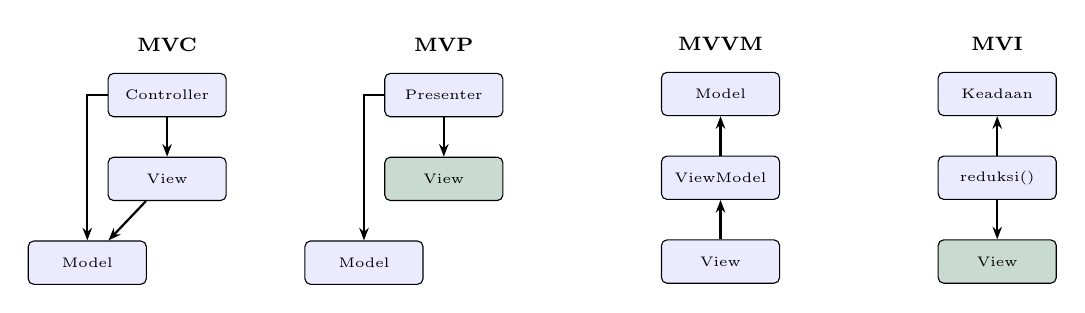
\begin{tikzpicture}[
    kotak/.style={draw, rounded corners=2pt, minimum width=1.5cm,
      minimum height=0.55cm, align=center, font=\tiny},
    panah/.style={-{Stealth[length=1.6mm]}, thick},
    judul/.style={font=\scriptsize\bfseries}
  ]
    \node[kotak, fill=blue!8] (mvc_v) {View};
    \node[kotak, fill=blue!8, below left=0.5cm and -0.5cm of mvc_v] (mvc_m) {Model};
    \node[kotak, fill=blue!8, above=0.5cm of mvc_v] (mvc_c) {Controller};
    \node[judul, above=0.15cm of mvc_c] {MVC};
    \draw[panah] (mvc_c) -- (mvc_v);
    \draw[panah] (mvc_c.west) -| (mvc_m.north);
    \draw[panah] (mvc_v) -- (mvc_m);

    \node[kotak, fill=praditagreen!25, right=2.0cm of mvc_v] (mvp_v) {View};
    \node[kotak, fill=blue!8, below left=0.5cm and -0.5cm of mvp_v] (mvp_m) {Model};
    \node[kotak, fill=blue!8, above=0.5cm of mvp_v] (mvp_p) {Presenter};
    \node[judul, above=0.15cm of mvp_p] {MVP};
    \draw[panah] (mvp_p) -- (mvp_v);
    \draw[panah] (mvp_p.west) -| (mvp_m.north);

    \node[kotak, fill=blue!8, right=2.0cm of mvp_v, yshift=-1.05cm] (mvvm_v) {View};
    \node[kotak, fill=blue!8, above=0.5cm of mvvm_v] (mvvm_vm) {ViewModel};
    \node[kotak, fill=blue!8, above=0.5cm of mvvm_vm] (mvvm_m) {Model};
    \node[judul, above=0.15cm of mvvm_m] {MVVM};
    \draw[panah] (mvvm_v) -- (mvvm_vm);
    \draw[panah] (mvvm_vm) -- (mvvm_m);

    \node[kotak, fill=praditagreen!25, right=2.0cm of mvvm_v] (mvi_v) {View};
    \node[kotak, fill=blue!8, above=0.5cm of mvi_v] (mvi_r) {reduksi()};
    \node[kotak, fill=blue!8, above=0.5cm of mvi_r] (mvi_s) {Keadaan};
    \node[judul, above=0.15cm of mvi_s] {MVI};
    \draw[panah] (mvi_r) -- (mvi_s);
    \draw[panah] (mvi_r) -- (mvi_v);
  \end{tikzpicture}

  \vspace{6pt}
  {\small Kotak hijau menandai View yang tidak bergantung pada komponen mana pun.}
\end{frame}

\begin{frame}{{\Large MVC Klasik: Model yang Memberi Tahu}}
  \vspace{4pt}
  \begin{center}
    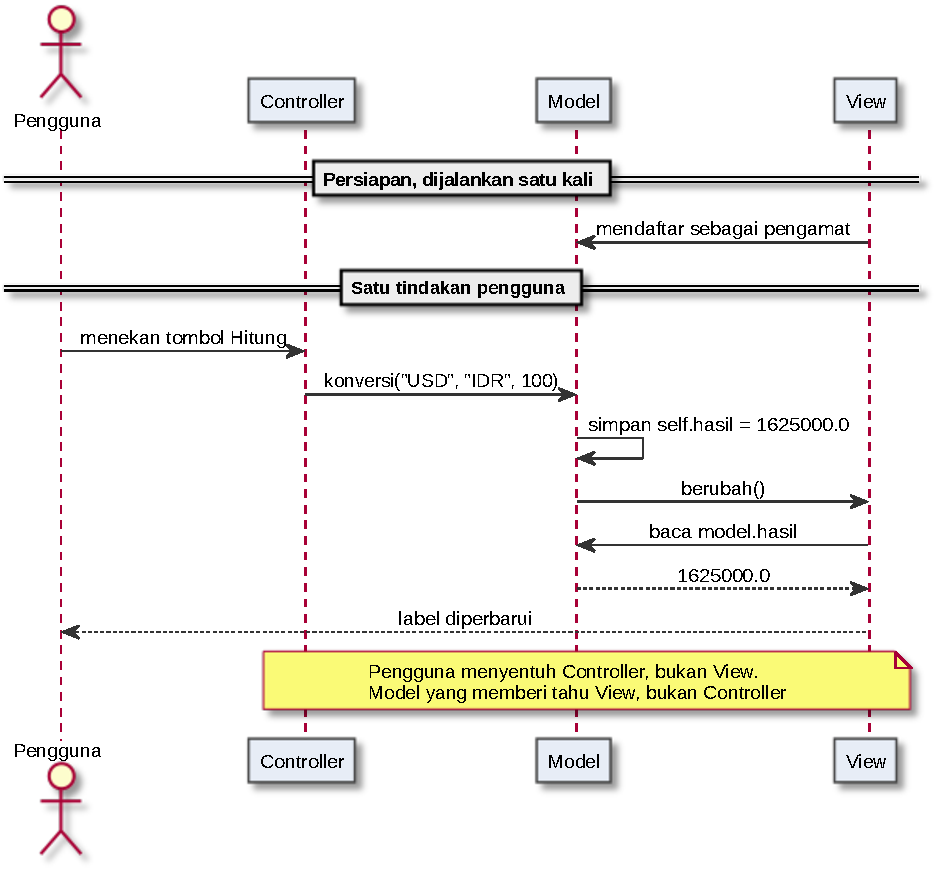
\includegraphics[width=\textwidth, height=0.72\textheight,
      keepaspectratio]{sekuens-mvc-klasik.pdf}
  \end{center}
\end{frame}

\begin{frame}[fragile]{{\Large MVC Masa Kini: View Membaca Model}}
  \vspace{12pt}
  \begin{columns}[T]
    \begin{column}{0.44\textwidth}
      \centering
      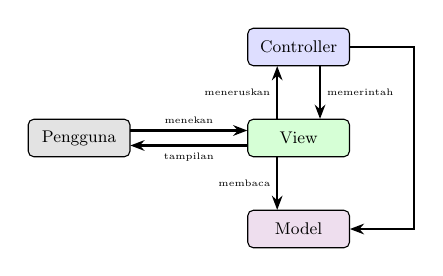
\begin{tikzpicture}[scale=0.68, transform shape,
        kotak/.style={draw, rounded corners=2pt, minimum width=1.9cm,
          minimum height=0.7cm, align=center, font=\small},
        panah/.style={-{Stealth[length=1.8mm]}, thick}
      ]
        \node[kotak, fill=cPenghubung] (c) at (0,0) {Controller};
        \node[kotak, fill=cView] (v) at (0,-1.7) {View};
        \node[kotak, fill=cModel] (m) at (0,-3.4) {Model};
        \node[kotak, fill=cPengguna] (u) at (-4.1,-1.7) {Pengguna};
        \draw[panah] ([yshift=1.4mm]u.east) -- ([yshift=1.4mm]v.west)
          node[midway, above, font=\tiny] {menekan};
        \draw[panah] ([yshift=-1.4mm]v.west) -- ([yshift=-1.4mm]u.east)
          node[midway, below, font=\tiny] {tampilan};
        \draw[panah] ([xshift=-4mm]v.north) -- ([xshift=-4mm]c.south)
          node[midway, left, font=\tiny] {meneruskan};
        \draw[panah] ([xshift=4mm]c.south) -- ([xshift=4mm]v.north)
          node[midway, right, font=\tiny] {memerintah};
        \draw[panah] ([xshift=-4mm]v.south) -- ([xshift=-4mm]m.north)
          node[midway, left, font=\tiny] {membaca};
        \draw[panah] (c.east) -- ++(1.2,0) |- (m.east);
      \end{tikzpicture}
    \end{column}
    \begin{column}{0.54\textwidth}
      \begin{itemize}\small
        \item Pengguna menyentuh View, lalu View meneruskannya ke Controller.
        \item Controller memanggil Model, lalu memerintah View menggambar.
        \item View membaca Model sendiri untuk mengambil nilainya.
        \item Ciri khasnya, \textbf{View mengenal Model}.
      \end{itemize}
      \vspace{3pt}
\begin{lstlisting}[style=PythonStyle]
class View:
  def __init__(self, induk, model):
    self.model = model   # ciri khas MVC
  def saat_ditekan(self):
    self.controller.tangani_masukan(...)
\end{lstlisting}
      \vspace{2pt}
      {\footnotesize Total ketergantungan 3, dan View butuh Model.}
    \end{column}
  \end{columns}
\end{frame}

\begin{frame}[fragile]{{\Large MVP: View Dibuat Pasif}}
  \vspace{12pt}
  \begin{columns}[T]
    \begin{column}{0.44\textwidth}
      \centering
      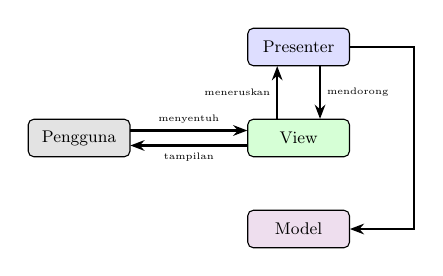
\begin{tikzpicture}[scale=0.68, transform shape,
        kotak/.style={draw, rounded corners=2pt, minimum width=1.9cm,
          minimum height=0.7cm, align=center, font=\small},
        panah/.style={-{Stealth[length=1.8mm]}, thick}
      ]
        \node[kotak, fill=cPenghubung] (p) at (0,0) {Presenter};
        \node[kotak, fill=cView] (v) at (0,-1.7) {View};
        \node[kotak, fill=cModel] (m) at (0,-3.4) {Model};
        \node[kotak, fill=cPengguna] (u) at (-4.1,-1.7) {Pengguna};
        \draw[panah] ([yshift=1.4mm]u.east) -- ([yshift=1.4mm]v.west)
          node[midway, above, font=\tiny] {menyentuh};
        \draw[panah] ([yshift=-1.4mm]v.west) -- ([yshift=-1.4mm]u.east)
          node[midway, below, font=\tiny] {tampilan};
        \draw[panah] ([xshift=-4mm]v.north) -- ([xshift=-4mm]p.south)
          node[midway, left, font=\tiny] {meneruskan};
        \draw[panah] ([xshift=4mm]p.south) -- ([xshift=4mm]v.north)
          node[midway, right, font=\tiny] {mendorong};
        \draw[panah] (p.east) -- ++(1.2,0) |- (m.east);
      \end{tikzpicture}
    \end{column}
    \begin{column}{0.54\textwidth}
      \begin{itemize}\small
        \item Pengguna menyentuh View, lalu View meneruskannya ke Presenter.
        \item Presenter menyusun seluruh teks tampilannya.
        \item View hanya menyimpan apa yang diberikan Presenter.
        \item \textbf{View tidak mengenal Model} sama sekali.
      \end{itemize}
      \vspace{3pt}
\begin{lstlisting}[style=PythonStyle]
class View:
  def tampilkan(self, teks):
    self.teks = teks
\end{lstlisting}
      \vspace{2pt}
      {\footnotesize Total ketergantungan 2, View butuh nol. Pengujian cukup
      memakai View tiruan.}
    \end{column}
  \end{columns}
\end{frame}

\begin{frame}[fragile]{{\Large MVVM: View Mengamati Properti}}
  \vspace{2pt}
  \begin{columns}[T]
    \begin{column}{0.36\textwidth}
      \centering
      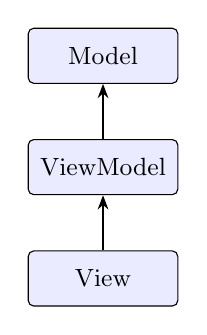
\begin{tikzpicture}[
        kotak/.style={draw, rounded corners=2pt, minimum width=1.9cm,
          minimum height=0.7cm, align=center, font=\small},
        panah/.style={-{Stealth[length=1.8mm]}, thick}
      ]
        \node[kotak, fill=blue!8] (m) {Model};
        \node[kotak, fill=blue!8, below=0.7cm of m] (vm) {ViewModel};
        \node[kotak, fill=blue!8, below=0.7cm of vm] (v) {View};
        \draw[panah] (vm) -- (m);
        \draw[panah] (v) -- (vm);
      \end{tikzpicture}
    \end{column}
    \begin{column}{0.54\textwidth}
      \begin{itemize}\small
        \item ViewModel menulis hasil ke properti yang dapat diamati.
        \item View mendaftar sebagai pengamat, lalu memperbarui dirinya.
        \item \textbf{ViewModel tidak mengenal View}, sehingga arahnya satu.
      \end{itemize}
      \vspace{3pt}
\begin{lstlisting}[style=PythonStyle]
class View:
  def __init__(self, view_model):
    view_model.teks.amati(self.saat_berubah)
\end{lstlisting}
      \vspace{2pt}
      {\footnotesize Total ketergantungan 3, sama dengan MVC, tetapi arahnya
      berbeda. Pengujian cukup membaca propertinya.}
    \end{column}
  \end{columns}
\end{frame}

\begin{frame}[fragile]{{\Large MVI: Penghubungnya Sebuah Fungsi}}
  \vspace{2pt}
  \begin{columns}[T]
    \begin{column}{0.36\textwidth}
      \centering
      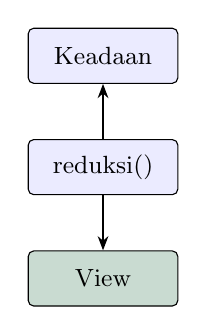
\begin{tikzpicture}[
        kotak/.style={draw, rounded corners=2pt, minimum width=1.9cm,
          minimum height=0.7cm, align=center, font=\small},
        panah/.style={-{Stealth[length=1.8mm]}, thick}
      ]
        \node[kotak, fill=blue!8] (s) {Keadaan};
        \node[kotak, fill=blue!8, below=0.7cm of s] (r) {reduksi()};
        \node[kotak, fill=praditagreen!25, below=0.7cm of r] (v) {View};
        \draw[panah] (r) -- (s);
        \draw[panah] (r) -- (v);
      \end{tikzpicture}
    \end{column}
    \begin{column}{0.54\textwidth}
      \begin{itemize}\small
        \item Setiap tindakan pengguna dibungkus menjadi Intent.
        \item Fungsi reduksi mengubah keadaan lama menjadi keadaan baru.
        \item Keadaannya tidak dapat diubah, sehingga riwayat dapat diputar
              ulang.
      \end{itemize}
      \vspace{3pt}
\begin{lstlisting}[style=PythonStyle]
def reduksi(keadaan, intent):
  hasil = domain.hitung_konversi(...)
  return replace(keadaan, teks=...)
\end{lstlisting}
      \vspace{2pt}
      {\footnotesize Total ketergantungan 0, sebab penghubungnya fungsi, bukan
      kelas yang menyimpan rujukan.}
    \end{column}
  \end{columns}
\end{frame}

\begin{frame}{{\Large Siapa Memakai Varian yang Mana}}
  \vspace{6pt}
  \begin{center}\small
  \begin{tabular}{|l|p{6.6cm}|}
    \hline
    \textbf{Varian} & \textbf{Contoh produk} \\
    \hline
    MVC klasik & Smalltalk-80 \\
    \hline
    MVC masa kini & Ruby on Rails, Laravel, Spring MVC, ASP.NET Core MVC \\
    \hline
    MVP & Google Web Toolkit, Windows Forms, Android sebelum Jetpack \\
    \hline
    MVVM & Windows Presentation Foundation, .NET MAUI, Vue.js versi awal \\
    \hline
    MVI & Redux, arsitektur Elm, Flutter Bloc \\
    \hline
  \end{tabular}
  \end{center}
\end{frame}

\begin{frame}{{\Large Tiga Sebutan yang Sering Keliru}}
  \vspace{6pt}
  \begin{itemize}\small
    \item \textbf{Django bukan MVC menurut namanya sendiri.} Django menyebut
      polanya MTV, yaitu \textit{Model-Template-View}. Berkas \texttt{views.py}
      berperan sebagai Controller, sedangkan templatnya berperan sebagai View.
    \item \textbf{Android tidak menyebut dirinya MVVM.} Dokumentasi resminya
      menyebut \texttt{ViewModel} sebagai \textit{state holder} di dalam
      susunan berlapis, dan istilah MVVM tidak dipakai sama sekali.
    \item \textbf{Redux mewarisi arsitektur Elm.} Fungsi pembaruan pada Elm
      bertanda tangan \texttt{(action, state) => state}, dan fungsi tersebut
      sama perannya dengan fungsi reduksi.
  \end{itemize}
  \vspace{4pt}
  {\footnotesize Penyebutan pola berubah seiring versi. Rujukan versi karena itu
  perlu ikut dicatat.}
\end{frame}

\begin{frame}{{\Large Satu Gagasan Bernama Intent}}
  \vspace{14pt}
  {\small Intent untuk mengirim pesan singkat tidak mengirim apa pun sendiri.
  Objek tersebut hanya menyatakan niat.}
  \vspace{5pt}
  \begin{center}\footnotesize
  \begin{tabular}{|l|p{3.7cm}|p{3.5cm}|}
    \hline
    \textbf{Hal} & \textbf{Intent pada Android} & \textbf{Intent pada MVI} \\
    \hline
    Gagasannya & Niat dibungkus menjadi objek data & Niat dibungkus menjadi objek data \\
    \hline
    Tujuannya & Ada keadaan berubah atau proses dijalankan & Ada keadaan berubah atau proses dijalankan \\
    \hline
    Penyalurnya & Sistem operasi Android & Fungsi reduksi \\
    \hline
    Cakupannya & Melintasi komponen dan aplikasi & Di dalam satu layar \\
    \hline
  \end{tabular}
  \end{center}
  \vspace{3pt}
  {\footnotesize Gagasannya sama, dan namanya \textit{command}. Yang berbeda
  hanya tingkat penerapannya, sehingga memakai \texttt{Intent} belum berarti
  memakai MVI.}
\end{frame}

\begin{frame}{{\Large Analogi: Dua Petugas Loket}}
  \vspace{10pt}
  \begin{itemize}
    \item Petugas pertama harus membuka lemari arsip sendiri untuk menjawab.
    \item Petugas kedua hanya membacakan lembar yang sudah disiapkan bagian
          lain.
    \item Petugas pertama sulit digantikan, sebab penggantinya harus mengenal
          isi lemari.
    \item Petugas kedua mudah digantikan siapa pun.
  \end{itemize}

  \vspace{10pt}
  {\small View pada MVC berperan seperti petugas pertama, sedangkan View pada
  MVP dan MVI berperan seperti petugas kedua.}
\end{frame}

\begin{frame}{{\Large Kasus: Menguji Layar yang Tidak Dapat Dijalankan}}
  \vspace{8pt}
  \begin{enumerate}
    \item Tim ingin menguji aturan penolakan nominal nol.
    \item Pada MVC, pengujian tetap menuntut objek View dibuat lebih dahulu.
    \item View menuntut Model, dan Model menuntut sambungan data.
    \item Pengujian akhirnya menyalakan hampir seluruh aplikasi.
    \item Pada MVI, pengujian cukup memanggil satu fungsi reduksi.
  \end{enumerate}

  \vspace{8pt}
  {\small Yang menentukan bukan jumlah kelasnya, melainkan komponen apa yang
  dituntut View.}
\end{frame}

\begin{frame}{{\Large Hasil Pengukuran}}
  \vspace{8pt}
  \centering
  \begin{tabularx}{0.95\textwidth}{|l|l|l|X|}
    \hline
    \textbf{Varian} & \textbf{Total} & \textbf{View butuh} & \textbf{Cara pengujian} \\
    \hline
    MVC & 3 & Model & Membutuhkan View asli \\
    \hline
    MVP & 2 & tidak ada & Cukup View tiruan \\
    \hline
    MVVM & 3 & ViewModel & Tanpa View, cukup membaca propertinya \\
    \hline
    MVI & 0 & tidak ada & Tanpa View, cukup memanggil fungsi reduksi \\
    \hline
  \end{tabularx}

  \vspace{10pt}
  {\small MVC dan MVVM mencatat total yang sama, tetapi arahnya berbeda. Angka
  perlu dibaca bersama arahnya.}
\end{frame}

\begin{frame}[fragile]{{\Large Ketika Satu Komponen Menggemuk}}
  \vspace{4pt}
  {\small Pemisahan peran hanya bertahan bila setiap komponen menolak pekerjaan
  yang bukan miliknya.}
  \vspace{4pt}
\begin{lstlisting}[style=PythonStyle]
class Controller:            # fat controller
  def tangani_masukan(self, asal, tujuan, nominal):
    if nominal <= 0:                    # aturan bisnis
      return "Galat: nominal harus positif"
    hasil = nominal * self.model.cari_kurs(asal, tujuan)
    return f"Hasil: {hasil:,.2f}"       # penyusunan tampilan
\end{lstlisting}
  \vspace{2pt}
  \begin{itemize}\small
    \item Aturan tersebut tidak dapat dipakai ulang oleh pintu masuk lain.
    \item Pengujiannya menuntut konteks permintaan, padahal isinya hanya
      perkalian dan perbandingan angka.
  \end{itemize}
\end{frame}

\begin{frame}{{\Large Tiga Gejala dan Perbaikannya}}
  \vspace{6pt}
  \begin{center}\footnotesize
  \begin{tabular}{|l|p{3.9cm}|p{3.7cm}|}
    \hline
    \textbf{Gejala} & \textbf{Tanda yang terlihat} & \textbf{Perbaikan} \\
    \hline
    Fat controller & Validasi dan perhitungan ada di Controller & Pindahkan aturannya ke Model \\
    \hline
    Fat model & Satu kelas mengurus aturan, basis data, dan format & Bagi menurut alasan berubahnya \\
    \hline
    Fat view & Percabangan dan perhitungan ada di templat & Susun teksnya di Presenter \\
    \hline
  \end{tabular}
  \end{center}
  \vspace{4pt}
  {\footnotesize \texttt{periksa\_mv.py} mengukur arah ketergantungan, bukan
  ukuran komponennya. Arah panah yang benar belum menjamin pembagian kerja yang
  sehat.}
\end{frame}

\begin{frame}{{\Large Ringkasan}}
  \vspace{12pt}
  \begin{itemize}
    \item Seluruh varian memisahkan tampilan dari aturan bisnis. Yang berbeda
          hanyalah cara penghubungnya bekerja.
    \item Pembeda yang menentukan adalah komponen yang dikenal View. Semakin
          sedikit yang dikenal, semakin mudah diuji tanpa antarmuka.
    \item Jumlah ketergantungan saja tidak cukup, sebab arahnya ikut
          menentukan.
    \item Arah panah yang benar pun belum menjamin pembagian kerja yang sehat,
          sebab satu komponen tetap dapat menggemuk.
  \end{itemize}
\end{frame}

\begin{frame}[fragile]{{\Large Persiapan Latihan}}
  \vspace{5pt}
\begin{lstlisting}[language=bash]
# sekali saja, dari akar repositori
bash sources/siapkan_venv.sh
source .venv/bin/activate
python -c "import tkinter"

cd sources/chapter03
python mvc.py
\end{lstlisting}

  \vspace{5pt}
  {\small Latihan bab ini menampilkan jendela, sehingga modul \texttt{tkinter}
  harus tersedia. Pada Debian dan Ubuntu, modulnya ada di paket
  \texttt{python3-tk}. Satu aplikasi, empat varian, tiga masalah berbeda.}
\end{frame}

\begin{frame}[fragile]{{\Large Latihan 1: Memetakan Ketergantungan}}
  \vspace{3pt}
\begin{lstlisting}[language=bash]
python periksa_mv.py
\end{lstlisting}

  \vspace{3pt}
  \begin{enumerate}
    \item Catat baris \texttt{Total ketergantungan} dan \texttt{Ketergantungan
          View} untuk keempat varian.
    \item Buka keempat berkas, lalu tunjukkan baris konstruktor yang menjadi
          sumber setiap ketergantungan.
    \item Gambarkan arah panah antar komponen untuk keempat varian.
  \end{enumerate}

  \vspace{3pt}
  {\small Pertanyaan: MVC dan MVVM mencatat total yang sama. Mengapa keduanya
  tetap berbeda sifatnya?}
\end{frame}

\begin{frame}[fragile]{{\Large Latihan 2: Menguji Tanpa Antarmuka}}
  \vspace{3pt}
\begin{lstlisting}[language=bash]
python uji_tanpa_antarmuka.py
\end{lstlisting}

  \vspace{3pt}
  \begin{enumerate}
    \item Catat cara uji yang dipakai setiap varian.
    \item Bandingkan isi keempat fungsi ujinya.
    \item Coba tulis ulang pengujian MVC tanpa membuat objek View, lalu catat
          apa yang menghalangi.
  \end{enumerate}

  \vspace{3pt}
  {\small Pertanyaan: cocokkan kolom cara uji dengan kolom ketergantungan View
  pada Latihan 1. Apa hubungan keduanya?}
\end{frame}

\begin{frame}[fragile]{{\Large Latihan 3: Mengukur Dampak Perubahan}}
  \vspace{3pt}
\begin{lstlisting}[language=bash]
git diff --stat mvc.py mvp.py mvvm.py mvi.py
\end{lstlisting}

  \vspace{3pt}
  \begin{enumerate}
    \item Catat perkiraan berkas yang akan berubah sebelum mulai menyunting.
    \item Tambahkan baris kedua yang menyebut nilai kurs pada keempat varian.
    \item Jalankan ulang pengujian untuk memastikan keempatnya masih berjalan.
    \item Hitung berkas, kelas, dan baris yang berubah.
  \end{enumerate}

  \vspace{3pt}
  {\small Pertanyaan: mengapa varian dengan ketergantungan paling sedikit belum
  tentu yang paling sedikit berubah?}
\end{frame}

\end{document}
